\section{Results}
\label{sec:results}
In this section we start with an overview of the bugs we identified in tiptop. Then, we follow with a discussion of our feature enhancements.

\subsection{Bug Fixes}
In our initial attempt to understand tiptop and its range of features we encountered an anomaly.
In some cases a question mark would appear, instead of a value from the hardware performance counter.
This would happen consistently for programs such as the Chrome~\cite{xxx} web browser, and would happen sporadically for other applications.
In Figure~\ref{fig:tiptop-bug} we have a screenshot that highlights this bug.

\begin{figure}[t]
\footnotesize
\centering
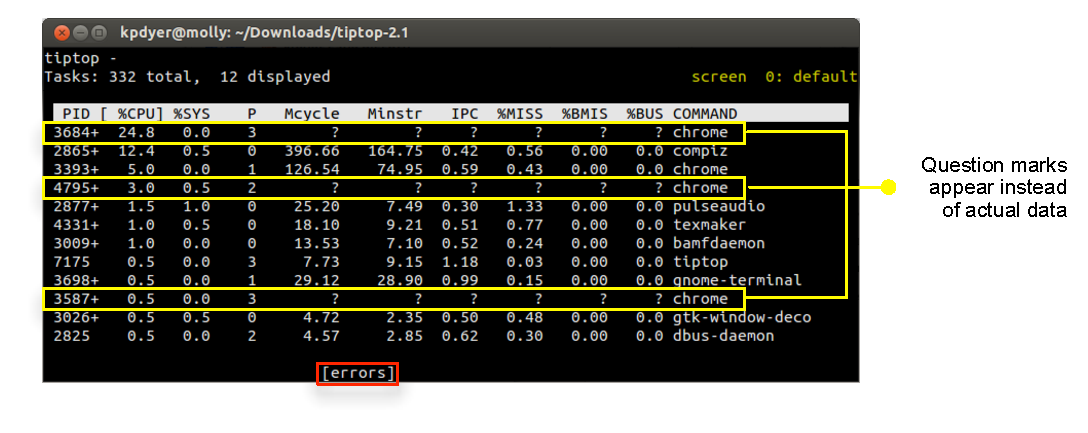
\includegraphics[width=.9\textwidth]{tiptop-bug}
%\hspace{.1in}
%\includegraphics[width=0.48\textwidth]{tiptop-default-screenshot-1}
\caption{A screenshot of the manifestation of the two bugs identified in our development. When tiptop is unable to determine the values associated with a process it ouputs a question mark instead. As we can see, tiptop failed to gather statistics for three of the four chrome processes in the above screenshot, at the bottom of the screen, in the red box, tiptop reports that \texttt{[errors]} occurred.}
\label{fig:tiptop-bug}
\end{figure}

Upon further investigation, we identified two separate issues that lead to this error condition.

\paragraph{Bug 1: Too many open file descriptors.}
First, a bit of background. Linux systems include a \texttt{limits.conf} file which enables a systems administrator to have fine-grained control over the system resources used by users and groups.
As an example, it is possible to specify the maximum priority of a process run by a specific user or group, or even the maximum number of processes spawned by a specific user or group. Each resource has a \emph{hard} and \emph{soft} limit. Hard limits are enforced by the kernel and can only be modified by superusers. Soft limits are default values and can be manually raised per-user, up to the hard limit.
For example, Ubuntu 12.04 has a soft limit of 1024 open file descriptors per user, and a hard limit of 4096.
This means that a regular user can open up to 1024 file descriptors under normal circumstances, or can open up to 4096 file descriptors by explicitly requesting (to the kernel) for the soft limit to be increased to 4096.

In order to read hardware counters, tiptop opens five counters per process in its default configuration.
For each combination of process and hardware counter, a file descriptor is opened.
As we can can see in the screenshot for Figure~\ref{fig:tiptop-bug}, my desktop had 332 running processes.
Hence, we now have a problem.
We have 332 processes, five hardware counters per process, so we have exceeded our soft limit for the number of file handlers open by requesting to open $332\cdot 5 = 1660$ file descriptors.

As a stopgap solution to this problem, we explicitly request for our soft file descriptor limit to be increased to the hard limit. This may be performed by fetching the hard limit from \texttt{/proc/N/limits}, then making a call to the \texttt{setrlimit} function, which is provided by \texttt{sys/resource.h}.
Unfortunately, increasing the open file descriptor limit beyond the hard limit requires superuser permission, which is undesirable.
Our solution to this problem is consistent with other open source project that have encountered this issue, such as Wine\footnote{\texttt{\url{https://bugs.launchpad.net/ubuntu/+source/linux/+bug/663090}}}.
A more robust solution for this bug is an open problem and would require fundamental changes to the design of tiptop, we talk about possible solutions in section~\ref{sec:conclusion}.

The testing for this was not straightforward due to a different bug, which we will discuss next.
In order to test this bug we ran tiptop as root, with root having a hard number of file descriptor set to 4096 and soft set to 1024. (By default, root has a soft limit of 4096 and hard limit of 8192 on Ubuntu 12.04.)
We may then run the version of tiptop that uses the soft limit and we get the following output.
\begin{verbatim}
19884+   4.6   0.0    0        ?        ?     ?      ?      ?     ? chrome
...
19818+   0.5   0.5    0        ?        ?     ?      ?      ?     ? firefox
\end{verbatim}

Simultaneously, we run the enhanced version of tiptop that explicitly requests a file descriptor limit to be raised to the hard limit, and we get the following output.
\begin{verbatim}
19884+   4.3   0.0    0 19327.35 19327.35  1.00   0.00   0.00   0.0 chrome
...
19818+   0.5   0.5    0  8589.93  8589.93  1.00   0.00   0.00   0.0 firefox
\end{verbatim}

We verify by that this bug is solved by checking that no value in the tiptop output has a question mark. Indeed, this solution is not robust, because other bugs may result in an error, which results in a failure to output process statistics, as we will see next.
In the final version of this project we hope to improve the robustness of our tests, such that error conditions are not conflated. We anticipate that this will require enhancements to tiptop's error reporting mechanism.

\paragraph{Bug 2: \texttt{EACCES}, permission denied.}
A second cause of ``questions marks" in the tiptop output has been traced to an \texttt{EACCES} permission denied error returned by the kernel, and is isolated to only a few applications, such as \texttt{chrome} and the \texttt{gnome-keyring-daemon}, to name a few.
This condition only occurs when running tiptop as a regular user.
We contacted the lead developer of tiptop, Erven Rohou, in order to determine the cause of this problem.
This was an unknown bug and a temporary workaround is running tiptop as root.
We will have additional information about the cause this bug in the final version of our report.

\subsection{Feature Enhancements}
Next, we will discuss the feature enhancements for tiptop.
First, we will discuss our enhancement to the default tiptop screen, which now includes the number of threads per process.
Then, we will discuss our integration with the cross-platform Performance Application Programming Interface (PAPI)~\cite{xxx} library.

\subsubsection{Thread count on main screen}
The primary focus for tiptop is a window to hardware counters.
However, there are other variables that can indirectly influence hardware performance.
As an example, say a developer wants to investigate the effect of inter-thread cache contention on the performance of their application.
Especially in cases when the number of threads in a process is not deterministic, it would be valuable to have the number of threads in a process on the tiptop screen. 
Therefore, we enabled tiptop to display the number of threads per process, and we included this feature on the default screen.

In our implementation we added hooks to the XML configuration logic to enable the ability to display the number of threads per process.
This involved adding code at multiple layers, including a call that exposed thread count from the data-gather layer to the presentations layer.
In addition, tiptop has multiple modes, which influence the filter that is applied to the processes/threads to be displayed.
As an example, tiptop can be run with the \texttt{-H} in order to show per-thread information, rather than per-process.
In such a case we do not want to display thread count, and our implementation includes logic such that thread count only appears in the case when we filter by processes.

In the testing of this feature we did the following, using Python and C.
\begin{enumerate}
\item Start a long-running C process that spawns $N$ threads.
\item Start tiptop in batch mode.
\item Verify that tiptop displays $N$ threads for the long-running C process.
\item Terminate long-running C process.
\end{enumerate}

Indeed, our test for this case is not robust. We are not testing multiple thread libraries, and we have tested this on only two platforms.
For the final version of this report we hope to include further details on strategies for increasing the robustness of these tests.

\begin{figure}[t]
\footnotesize
\centering
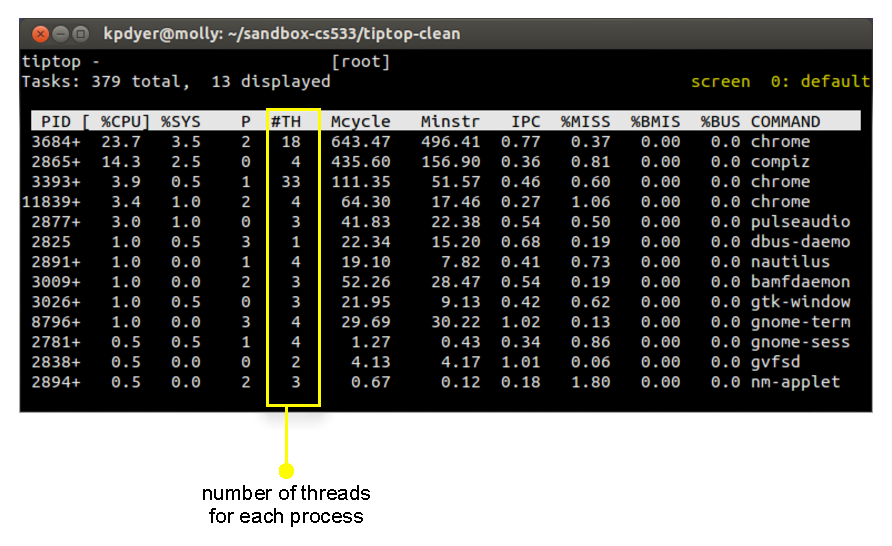
\includegraphics[width=.7\textwidth]{tiptop-threads}
%\hspace{.1in}
%\includegraphics[width=0.48\textwidth]{tiptop-default-screenshot-1}
\caption{A screenshot of the enhanced tiptop homescreen, showing the number of threads in each process.}
\label{fig:tiptop-threads}
\end{figure}

\subsubsection{Integration with the PAPI library}
The Performance Application Programming Interface (PAPI) library is a cross-platform API for accessing hardware performance counter information.
Roughly, it is a interface that removes the complexity involved in accessing hardware performance counters.
Let us consider a concrete example.
The man page for tiptop gives the following example for a way to manually specify the counter for the number of issued mico-ops on Sandy Bridge:
\begin{verbatim}
  <counter alias="uops_issued" config="0x010e"
           type="RAW" arch="x86" model="06_2A" />
\end{verbatim}
which then requires an additional call to the counter alias
\begin{verbatim}
  <column header=" U Ops" format="%5.1f"
          desc="U Ops Issues" expr="uops_issued" />
\end{verbatim}

The values for \texttt{config} and \texttt{model} in the \texttt{counter} tag are hardware-specific, and requires that the user looks at documentation in order to implement an alias, which can then be used to construct a column in a custom tiptop screen.
Indeed, it is less than ideal that a user has to specify magic numbers for their CPU.
What is more, any change to the underlying hardware may require a complete change to the XML configuration file.
This is certainly a nightmare when developing a tiptop screen that may be used across multiple platforms.

\paragraph{PAPI to the rescue.}
Fortunately, PAPI makes life much easier.
Instead of having to specify a hardware-specific counter macro, then reference the macro for display, our new feature enables a user to specify the PAPI event directly.
There are approximately one hundred different counter events specified in PAPI 5.0.1, and our goal is to enable the user to call as many of those as possible from the tiptop screen configuration file.
As an example, the following declaration would be able to integrate directly into the tiptop XML file
\begin{verbatim}
  <column header=" U Ops" format="%5.1f"
          desc="U Ops Issues" expr="PAPI_FP_OPS" />
\end{verbatim}
It is then up to PAPI to determine the correct hooks for a hardware counter, and the burden is not on the user to identify magic numbers.
This is cross-platform, as far as PAPI supports the specific counter specified.
Hence, the user does not have to specify a custom hardware-specific \texttt{counter} macro, and a single XML file can be specified and deployed across multiple system.
In addition, this is backwards compatible with previous versions of tiptop configurations files, and the prefix \texttt{PAPI\_} for an \texttt{expr} attribute in a \texttt{column} tag, is a flag for tiptop to call PAPI, rather than using a direct kernel call for hardware counters.

This feature is under development and we will have further information about the breadth of coverage of PAPI calls, and more information about our testing strategy.